\section{Calculated Sum-Frequency Spectra}

One of the aims of this simulation study is to complement our group's previous experimental SFG work.\cite{McFearing2009} The varied set of anions and their affect on the CCl$_4$-H$_2$O interface is linked from theory to empirical data through the connection of computed SFG spectra. The computed SFG spectra for each system are presented in figure \ref{fig:sfg-spectra} along with the experimental spectra from our previous work with these same salt solutions.\cite{McFearin2009} On first look, the overall intensities and lineshapes follow remarkably similar trends as in the experimental systems. The key features of the CCl$_4$-H$_2$O interfacial spectra are the diminished intensities below 3400 cm$^{-1}$ as compared to previous liquid-air works, and the dominant ``free-oh'' peak near 3660 cm$^{-1}$.

\begin{figure}[h!]
\begin{center}
	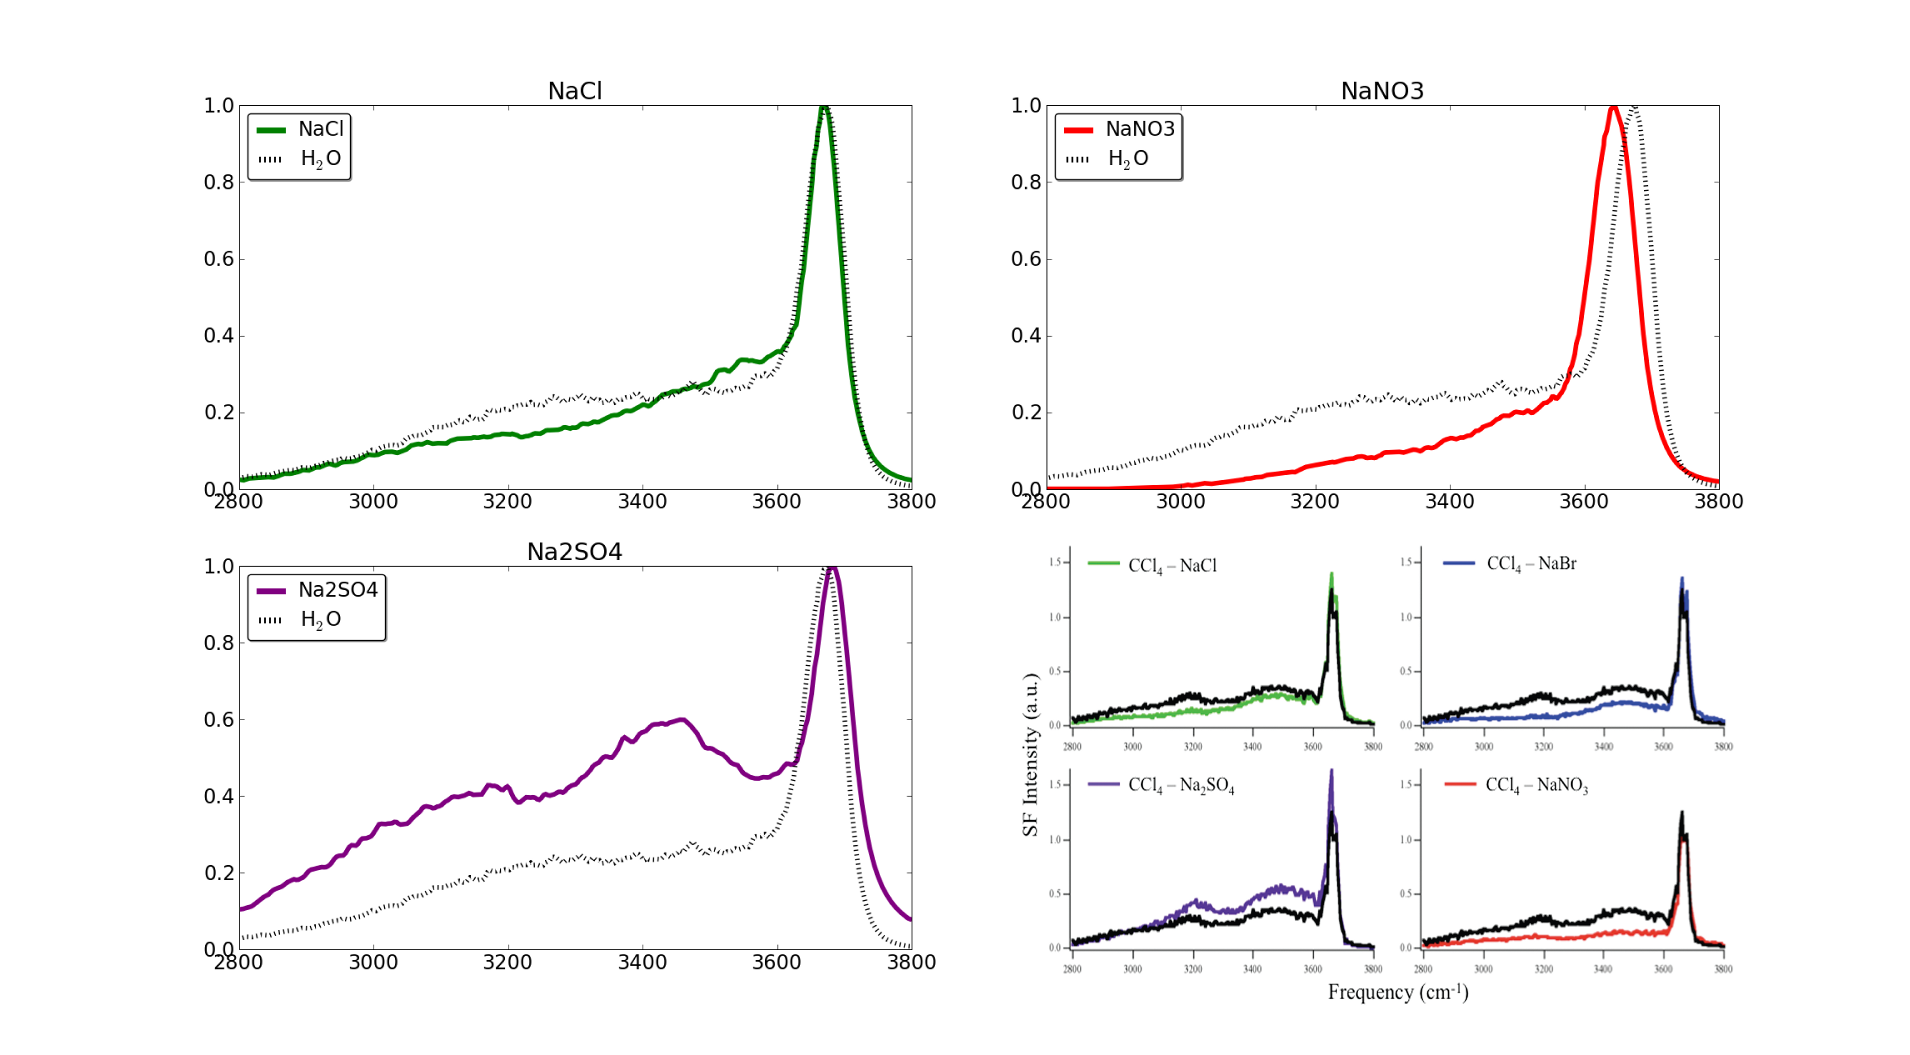
\includegraphics[scale=0.25]{images/sfg-spectra.png}
	\caption{Vibrational SFG spectra of the water-OH stretching region for each interfacial aqueous-salt/CCl$_4$ system. The water/CCl$_4$ interface spectrum (black-dashed line) is provided on the plot for each of the simulated systems for reference. The bottom-right figure is a reproduction of the experimental spectra from McFearin et al to show the intensity and lineshape trends found previously for these systems.\cite{McFearin2009}}
	\label{fig:sfg-spectra}
\end{center}
\end{figure}

The reference CCl$_4$-H$_2$O spectrum reproduces well the lineshape from experiment, but lacks the definition of the two peaks found near 3250 and 3450 cm$^{-1}$. These lower-frequency features have been attributed to the different H-bonding varieties of water that make up the more ``ice-like'' tetrahedral environments found deeper into the aqueous bulk. We have found similar trouble in reproducing the lower-frequency peaks near 3200 cm$^{-1}$, and attribute the slight differences in the lineshape to similar problems.\cite{Walker2006b} However, the lineshape is otherwise quite similar to that of the experiment, and warrants further comparison, and suggests that the methods are sound, and justified for this study.

For monovalent ions at the CCl$_4$-H$_2$O interface, the behavior is completely different than for the air-H$_2$O systems. Concentrations of monovalent anions were found to be lower at the CCl$_4$-H$_2$O interface than at the air-liquid one.\cite{Wick2007a} Larger and more polarizable anions were found to be less solvated than smaller ones such as Cl$^-$. I$^-$, for instance, has more contact with the CCl$_4$ phase because of a more exposed ion surface and higher polarizability, resulting in repulsion of the CCl$_4$ (and a wider aqueous interface), and decreased anion concentration.
